\documentclass[12pt, twoside]{article}
\usepackage[letterpaper, margin=1in, headsep=0.5in]{geometry}
\usepackage[english]{babel}
\usepackage[utf8]{inputenc}
\usepackage{amsmath}
\usepackage{amsfonts}
\usepackage{amssymb}
\usepackage{tikz}
\usetikzlibrary{quotes, angles}
\usepackage{graphicx}
\usepackage{enumitem}
\usepackage{multicol}

\newif\ifmeta
\metatrue %print standards and topics tags

\title{IB Mathematics}
\author{Chris Huson}
\date{September 2021}

\usepackage{fancyhdr}
\pagestyle{fancy}
\fancyhf{}
\renewcommand{\headrulewidth}{0pt} % disable the underline of the header
\raggedbottom


\fancyhead[LE]{\thepage}
\fancyhead[RO]{\thepage \\ Name: \hspace{4cm} \,\\}
\fancyhead[LO]{BECA / IB Math 01-Linear functions\\* 15 September 2021}

\begin{document}

\subsubsection*{1.3 Classwork: Linear equations prior knowledge}
\begin{enumerate}
\item In the following two problems, solve for the value of $x$.
  \begin{multicols}{2}
    \begin{enumerate}
      \item   $x-5=12$ \vspace{6cm}
      \item   $13-x=-3$ \vspace{6cm}
    \end{enumerate}
  \end{multicols}
    \vspace{2.5cm}

\item Given $g(x)=x^2-5x+15$. Simplify $g(0)$. \vspace{3cm}
\item Given $f(x)=3x-2$. Solve for $x$ such that for $f(x)=13$. \vspace{4cm}  

\item A line is shown on the grid below.
\begin{multicols}{2}
\begin{enumerate}
  \item Write down it's slope.\\ $m=$
  \vspace{0.25cm}
  \item Write down it's $y$-intercept.\\ $b=$
  \vspace{0.25cm}
  \item Write down the equation of the line.
  \vspace{1cm}
  \item State the coordinates of the point $P$.
\end{enumerate}
  \begin{center} %4 quadrant regents grid w T-Chart
  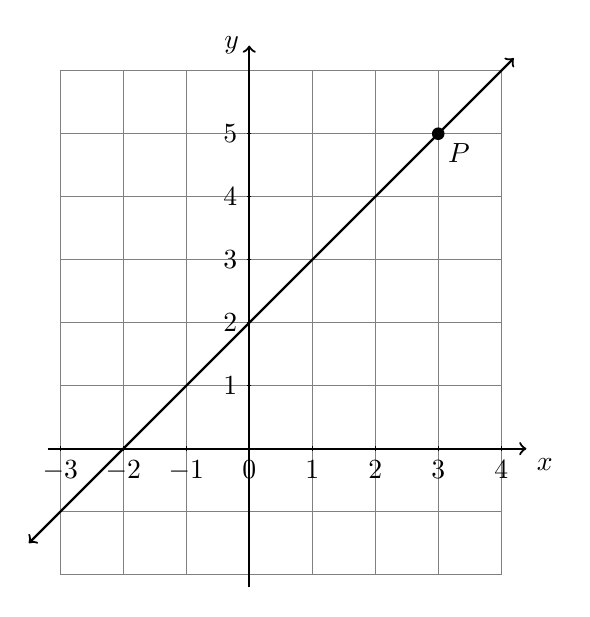
\begin{tikzpicture}[scale=0.8]
    \draw [help lines] (-3,-2) grid (4,6);
    \draw [thick, ->] (-3.2,0) -- (4.4,0) node [below right] {$x$};
    \draw [thick, ->] (0,-2.2)--(0,6.4) node [left] {$y$};
    \foreach \x in {-3, -2, ..., 4} \draw (\x cm,1pt) -- (\x cm,-1pt) node[anchor=north] {$\x$};
    \foreach \y in {1, 2, 3, 4, 5} \draw (1pt,\y cm) -- (-1pt,\y cm) node[anchor=east] {$\y$};
    \draw [thick, <->] (-3.5,-1.5) -- (4.2,6.2);
    \fill (3,5) circle[radius=0.1] node[below right]{$P$};
  \end{tikzpicture}
  \end{center}
\end{multicols}

\newpage
\item The line $l$ has the equation $y=\frac{3}{2}x-1$. 
\begin{enumerate}
  \item Write down it's slope. $m=$
  \vspace{0.5cm}
  \item Write down it's $y$-intercept. $b=$
  \vspace{0.5cm}
  \item Is the point $(4, 4)$ on the line $l$? Justify your answer.
\end{enumerate}
\vspace{2.5cm}

\item Draw a straight line through the points $A$ and $B$ shown on the grid below.
\begin{multicols}{2}
\begin{enumerate}
  \item Write down the line's $y$-intercept.\\ $b=$
  \vspace{0.25cm}
  \item Write down the slope of the line.\\ $m=$
  \vspace{0.25cm}
  \item Write down the equation of the line.
\end{enumerate}
  \begin{center} %4 quadrant regents grid w T-Chart
  \begin{tikzpicture}[scale=0.8]
    %\draw [help lines] (-3,-2) grid (4,6);
    \draw [thick, ->] (-3.2,0) -- (5.4,0) node [below right] {$x$};
    \draw [thick, ->] (0,-1.2)--(0,6.4) node [left] {$y$};
    \foreach \x in {-2, -1, ..., 5} \draw (\x cm,1pt) -- (\x cm,-1pt) node[anchor=north] {$\x$};
    \foreach \y in {1, 2, 3, 4, 5} \draw (1pt,\y cm) -- (-1pt,\y cm) node[anchor=east] {$\y$};
    %\draw [thick, <->] (-3.5,-1.5) -- (4.2,6.2);
    \fill (0,4) circle[radius=0.1] node[above right]{$A (0,4)$};
    \fill (4,2) circle[radius=0.1] node[above right]{$B (4,2)$};
  \end{tikzpicture}
  \end{center}
\end{multicols}
\vspace{2.5cm}

\item Early finishers: Simplify each expression. (Leave it in radical form if necessary, not a decimal.)
\begin{enumerate}
  \begin{multicols}{2}
  \item   $\sqrt{25}$ \vspace{1.5cm}
  \item   $\sqrt{24}$ \vspace{1.5cm}
  \end{multicols}
\end{enumerate}
\vspace{0.5cm}

\end{enumerate}
\end{document}